\documentclass{article}

\usepackage[utf8]{inputenc}	
\usepackage[english]{babel}
\usepackage[pangram]{blindtext}
\usepackage{lipsum}
\usepackage{graphicx}
\usepackage{epstopdf}
\graphicspath{{img/}}


\title{title}
\author{author}
\date{\today}

\begin{document}
	
	\maketitle
	\tableofcontents
%	\listoftables
	
	\section{Prima}
	Sezione principale 
	\subsection{Secondaria} 
	Sottosezione numerata 
	\subsection*{Un'altra secondaria} 
	Sottosezione non numerata 
	\section{Seconda}
	Seconda principale
	
	\clearpage
	
	\section*{Terza}
	\subsection*{Terza(1)}
	\begin{minipage}{.5\linewidth}
		\flushleft
		\textbf{Parte sinistra}\\
%		\Blindtext[1][3]
		\lipsum[66]
	\end{minipage}
	%\hspace{.4\linewidth}  % spazio orizzontale, dimensione specifica
	%\hfill % spazio orizzontale, riempimento
	\begin{minipage}{.5\linewidth}
		\flushright
		\textbf{Parte destra}\\
%		\Blindtext[1][3]
		\lipsum[66]
	\end{minipage}
	
	\subsection*{Terza(2)}
	\begin{minipage}{.33\linewidth}
		\flushleft
		\textbf{Parte sinistra}\\
		%		\Blindtext[1][3]
		\lipsum[66]
	\end{minipage}
%	\hspace{.4\linewidth}  % spazio orizzontale, dimensione specifica
%	\hfill % spazio orizzontale, riempimento
	\begin{minipage}{.33\linewidth}
		\flushright
		\textbf{Parte destra}\\
		%		\Blindtext[1][3]
		\lipsum[66]
	\end{minipage}
	
	\clearpage
	
	\section{Quarta}
	
	\blindtext	
	
	\begin{itemize}
		\item primo elemento
		\subitem sottoelemento
		\subsubitem sotto-sottoelemento
		\item[*] secondo elemento, bullet-point diverso
		\begin{enumerate}
			\item primo elemento (\verb|enumerate| annidato)
			\item secondo elemento (\verb|enumerate| annidato)
			\end{enumerate}
	\end{itemize}

	\blindtext

	\begin{description}
		\item[Nome] questo è il nome
		\item[Descrizione] questa è la descrizione 
	\end{description}
	
	\clearpage
	
	\section*{Quinta}
	
	\begin{table}[h]
		\centering
		\begin{tabular}{|c|c|c|}
			\hline
			1 & 2 & 3 \\ 
			\hline 
			4 & 5 & 6 \\ 
			\hline 
		\end{tabular}
	\caption{La nostra prima tabella ...}
	\label{tab:tab1}
	\end{table}
	
	\begin{table}[h]
	\centering
		\begin{tabular}{ | c c c c | r |}
		\cline{1-4}
		\multicolumn{4}{|c|}{Valori} &
		        \multicolumn{1}{l}{Somma} \\
		\hline
		7 & 5 & 3 & 4 & 19 \\ 2&1&3&3& 9\\ \hline
		\end{tabular} 
	\caption{Somme} 
	\label{tab:somme} 
	\end{table}\

	\clearpage

	\section*{Sesta}

	\Blindtext[1][3]

	\begin{figure}[h]
	\begin{center}
		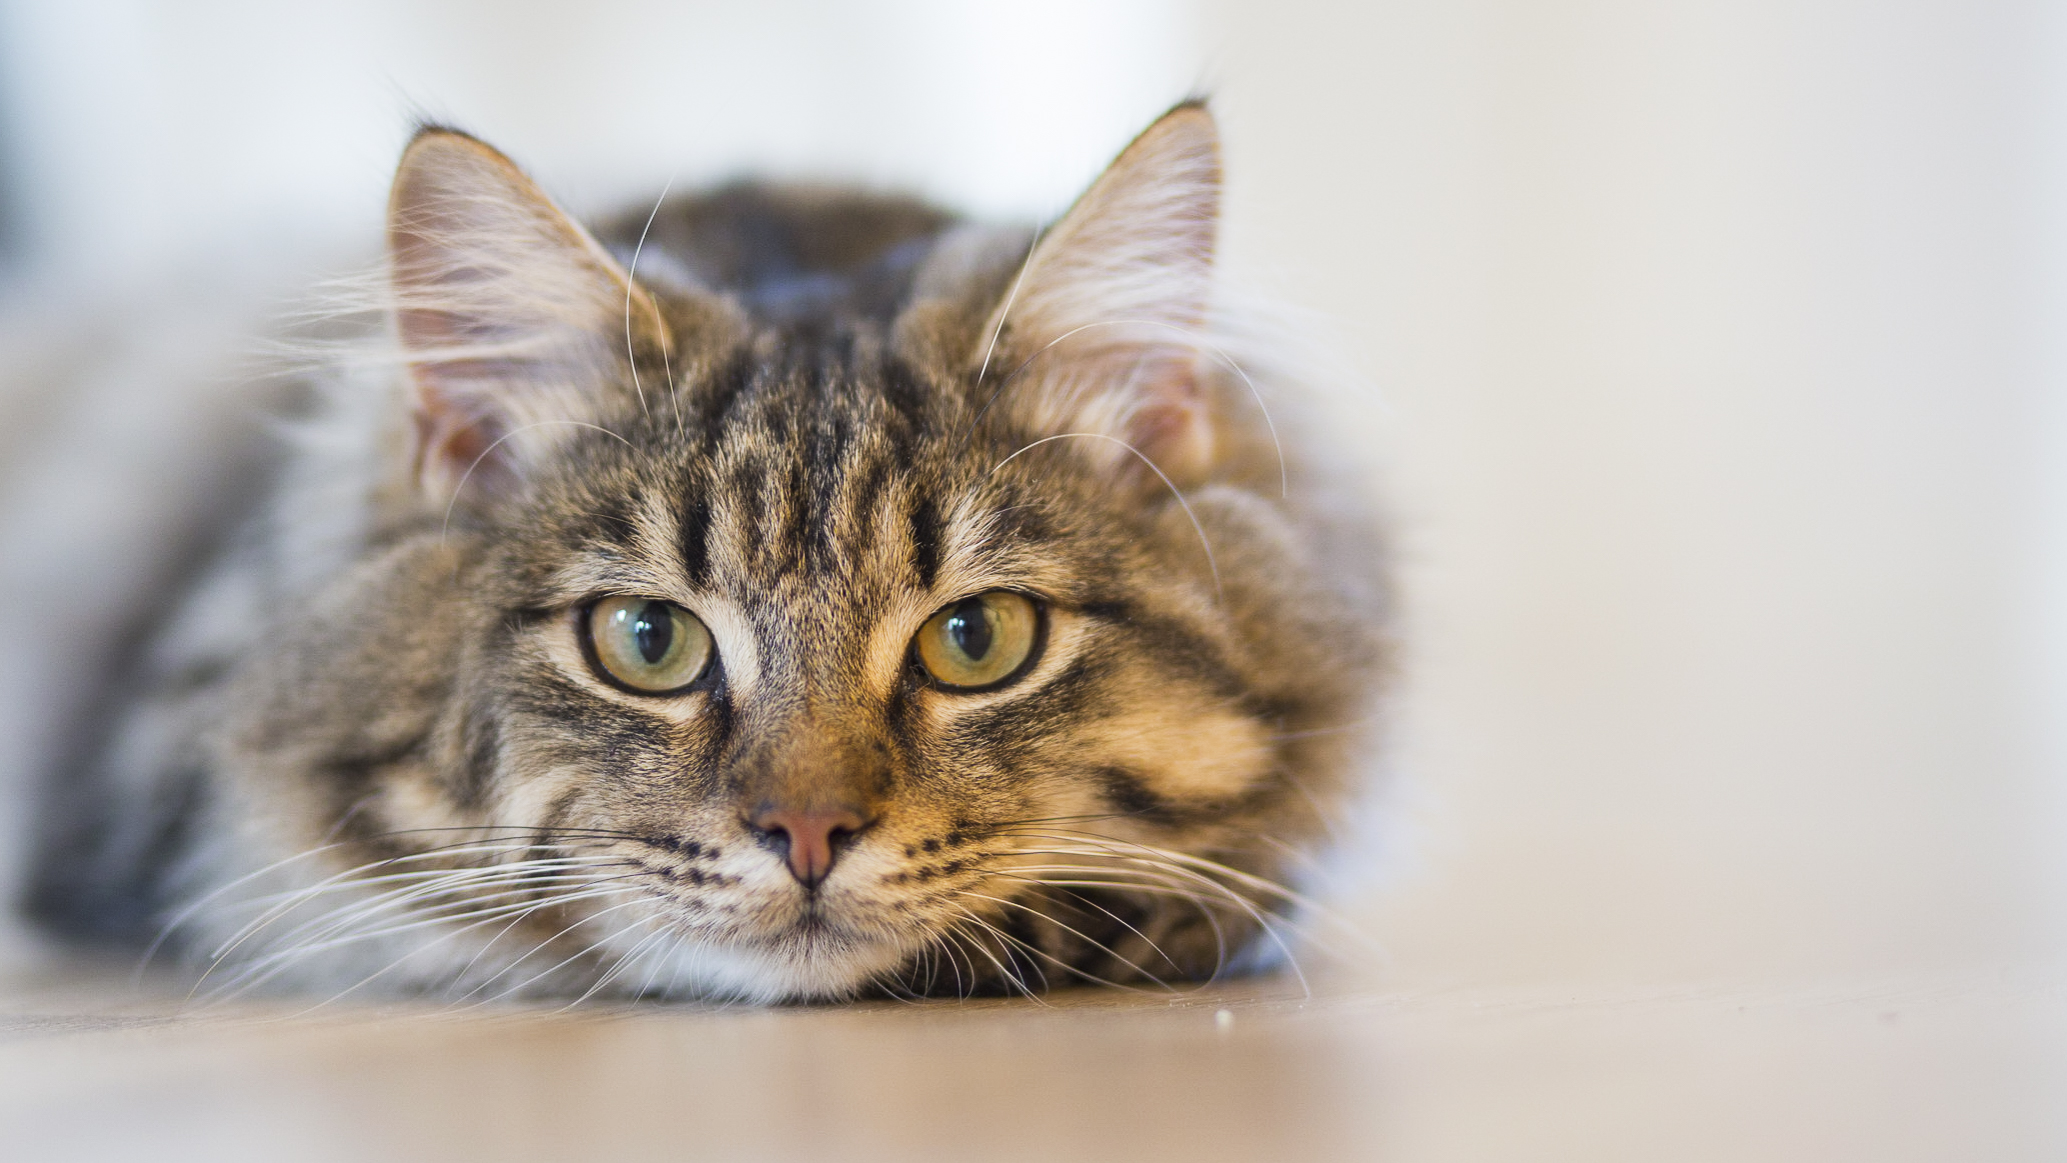
\includegraphics[width = .5\linewidth]{cat}
	\end{center}
	\caption{Un gatto}
	\label{fig:fig1}
	\end{figure}

	\Blindtext[1][3]
	
	\begin{figure}[h]
	\begin{center}
		\includegraphics[width = .5\linewidth]{eps_ex}
	\end{center}
	\caption{La prima immagine in .eps che ho trovato sull'internet}
	\label{fig:fig2}
	\end{figure}
	

\end{document}